%% This is an example first chapter.  You should put chapter/appendix that you
%% write into a separate file, and add a line \include{yourfilename} to
%% main.tex, where `yourfilename.tex' is the name of the chapter/appendix file.
%% You can process specific files by typing their names in at the 
%% \files=
%% prompt when you run the file main.tex through LaTeX.
\chapter{Menu-menu}  \label{chap:Menu}

\section{Manual}
Menu \emph{Manual} berisi \emph{link} untuk mendownload file Manual penggunaan Ijah Webserver. Kedepannya, isi file Manual juga akan ditampilkan di halaman ini.

\begin{figure}[H]
	\centering
	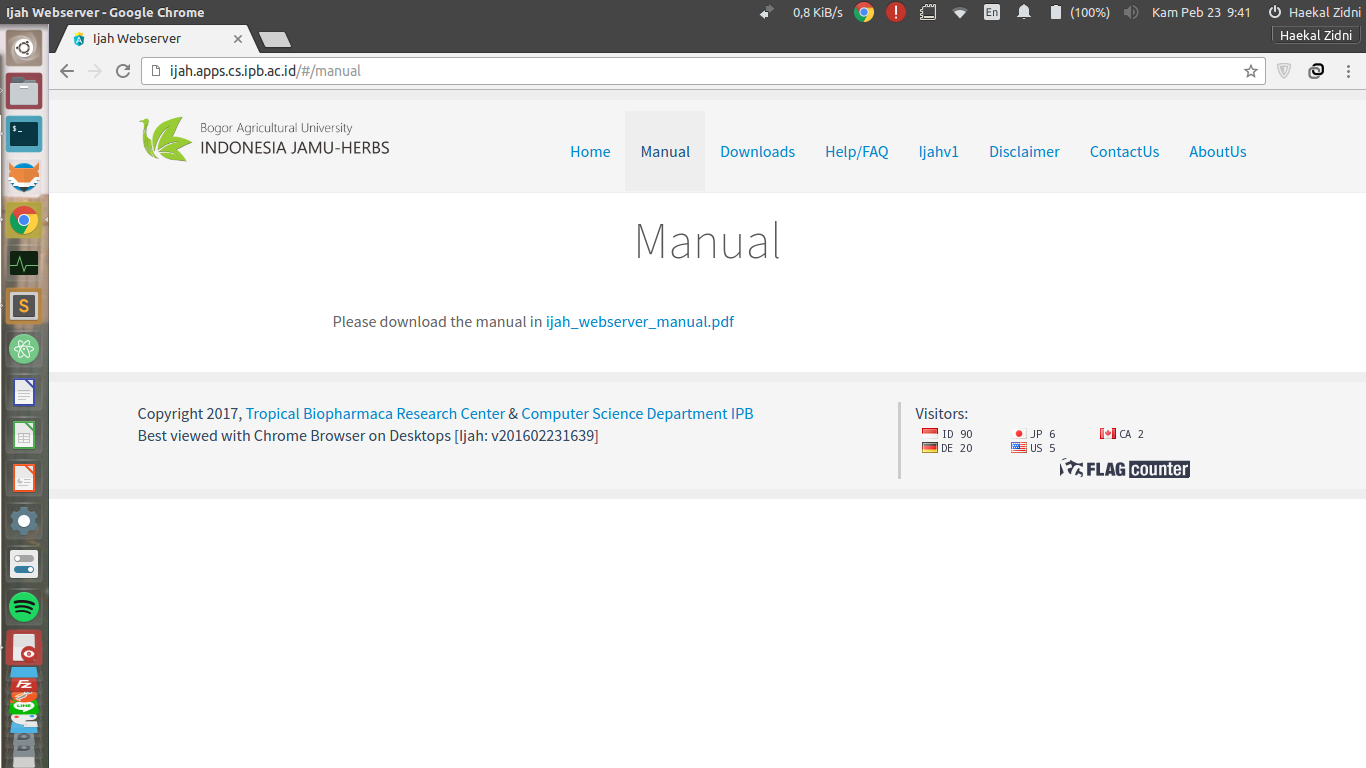
\includegraphics[scale=0.3]{ijah_manual_page.png}
	\caption{Halaman Manual}
	\label{fig:ijah_manual_page}
\end{figure}

\section{Downloads} \label{Downloads}
Menu \emph{Downloads} menyediakan link untuk mengunduh Metadata seluruh item (tanaman, senyawa, protein, dan penyakit) yang ada dalam database Ijah Webserver. Juga disediakan data seluruh konektivitas (keterhubungan) antar item dan data lainnya seperti similarity data, data sekuens protein, dan lain lain.

Untuk mengunduh file pada halaman ini cukup klik nama file yang ingin diunduh

\begin{figure}[H]
	\centering
	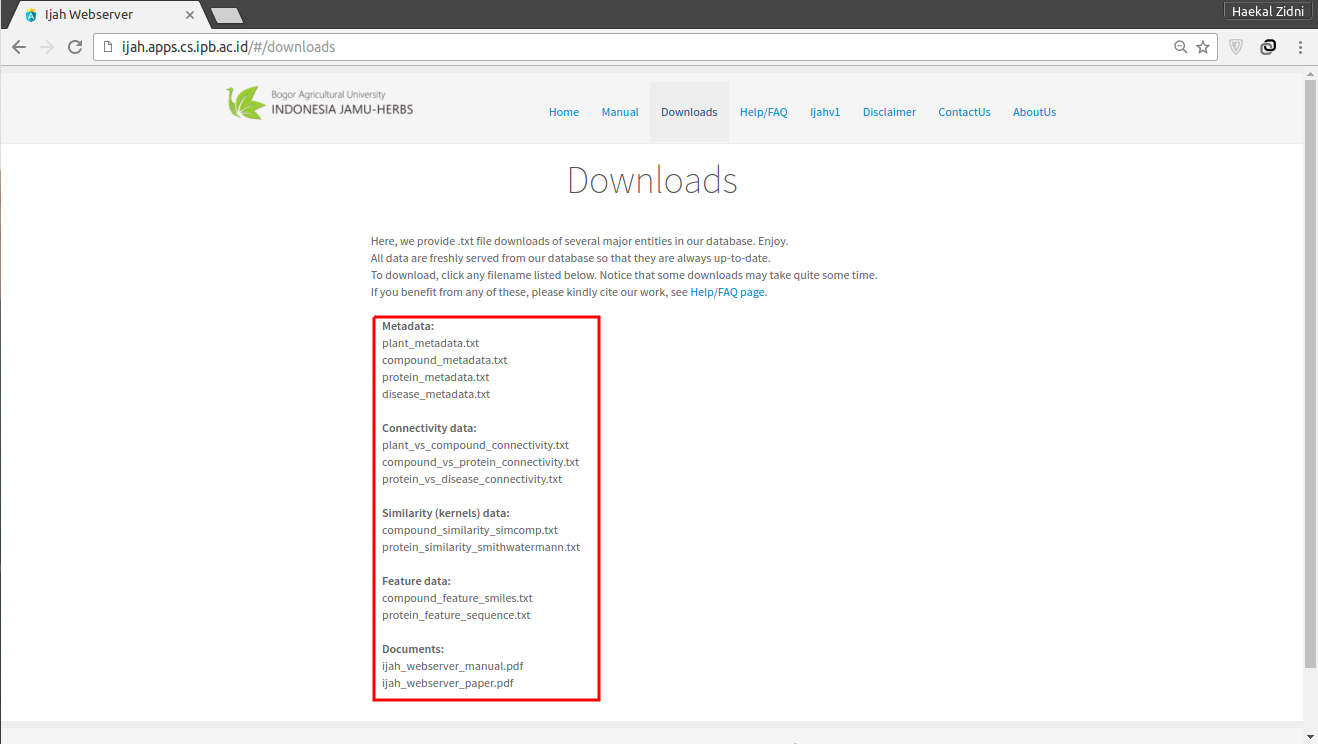
\includegraphics[scale=0.3]{ijah_downloadpage.png}
	\caption{Daftar file yang dapat di\-download}
	\label{fig:ijah_downloadpage}
\end{figure}

	\subsection{Metadata}
	File yang dapat didownload pada kategori Metadata yaitu:

	\begin{itemize}
	\item \textbf{plant\_metadata.txt} -- Berisi metadata seluruh tanaman pada \emph{database} Ijah Webserver. 
	\item \textbf{compound\_metadata.txt} -- Berisi metadata seluruh senyawa (\emph{compound}) pada \emph{database} Ijah Webserver.
	\item \textbf{protein\_metadata.txt} -- Berisi metadata seluruh bioprotein pada \emph{database} Ijah Webserver.
	\item \textbf{disease\_metadata.txt} -- Berisi metadata seluruh penyakit pada \emph{database} Ijah Webserver.
	\end{itemize}

	\subsection{Connectivity Data}
	File yang dapat didownload pada kategori Connectivity Data yaitu:

	\begin{itemize}
	\item \textbf{plant\_vs\_compound\_connectivity.txt} -- Berisi data konektivitas tanaman dengan senyawa beserta skor konektivitasnya pada \emph{database} Ijah Webserver.
	\item \textbf{compound\_vs\_protein\_connectivity.txt} -- Berisi data konektivitas senyawa dengan protein beserta skor konektivitasnya pada \emph{database} Ijah Webserver.
	\item \textbf{protein\_vs\_disease\_connectivity.txt} -- Berisi data konektivitas protein dengan penyakit beserta skor konektivitasnya pada \emph{database} Ijah Webserver.
	\end{itemize}

	\subsection{Similarity (kernels) data}
	\begin{itemize}
	\item compound\_similarity\_simcomp.txt  
	\item protein\_similarity\_smithwatermann.txt  
	\end{itemize}

	\subsection{Feature data}
	\begin{itemize}
	\item compound\_feature\_smiles.txt  
	\item protein\_feature\_sequence.txt  
	\end{itemize}

	\subsection{Documents}
	Dokumentasi Ijah Webserver
	\begin{itemize}
	\item \textbf{ijah\_webserver\_manual.pdf} -- Manual penggunaan Ijah Webserver
	\item \textbf{ijah\_webserver\_paper.pdf} -- Paper penelitian Ijah Webserver
	\end{itemize}

\section{Help/FAQ}
Menu \emph{Help/FAQ} berisikan beberapa pertanyaan umum \emph{(Frequently Asked Questions)} beserta jawabannya.

\begin{figure}[H]
	\centering
	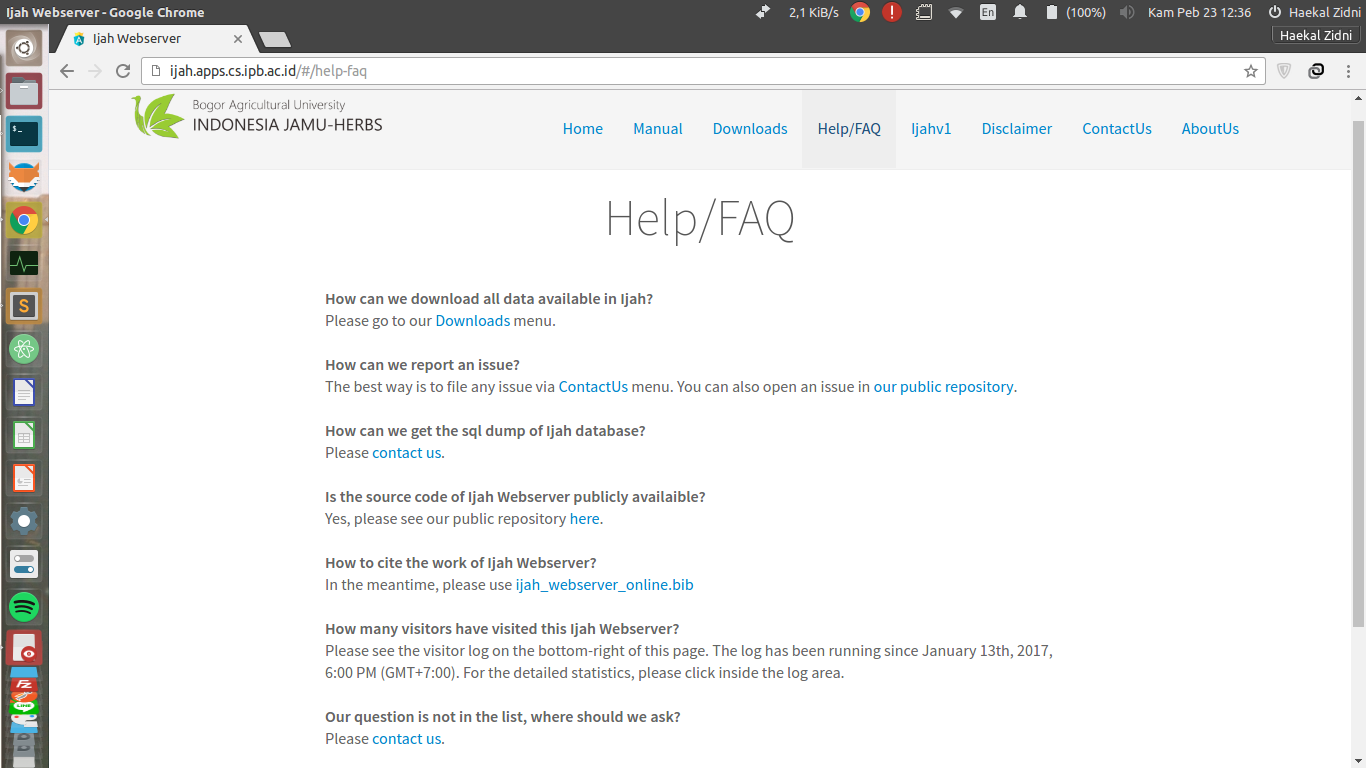
\includegraphics[scale=0.3]{ijah_faq.png}
	\caption{Halaman Help/FAQ}
	\label{fig:ijah_faq}
\end{figure}

Menu FAQ ini tersedia dalam bahasa Inggris, berikut terjemahan dari pertanyaan pada menu FAQ menurut Ijah Webserver versi ini:

\begin{itemize}
\item {\textbf{Q:}} Bagaimana cara mengunduh semua data yang ada pada Ijah?\\
A: Silakan menuju menu \textbf{\nameref{Downloads}}.
\item {\textbf{Q:}} Bagaimana cara melaporkan isu dan masalah?\\
A: Cara termudah yaitu dengan mengontak kami di menu \textbf{\nameref{ContactUs}}. Anda bisa juga menyampaikannya di repositori \emph{code} kami. (Menuju repositori -- lihat bab \ref{sec:ws_source}).
\item {\textbf{Q:}} Bagaimana cara mendapatkan \emph{SQL dump} dari \emph{database} Ijah?\\
A: Silakan kontak tim kami di menu \textbf{\nameref{ContactUs}}.
\item {\textbf{Q:}} Apakah \emph{source code} Ijah tersedia secara publik?\\
A: Ya, silakan lihat repositori publik kami disini (Menuju repositori -- silakan lihat bab \ref{sec:ws_source}).
\item {\textbf{Q:}} Bagaimana cara mengutip karya Ijah Webserver?\\
A: Untuk saat ini silakan lihat di \href{http://ijah.apps.cs.ipb.ac.id/api/ijah_webserver_online.bib}{\textbf{ijah\_webserver\_online.bib}}
\item {\textbf{Q:}} Berapa kali Ijah Webserver telah dikunjungi?\\
A: Silakan lihat \emph{visitor log} pada bagian kanan-bawah halaman Ijah Webserver. \emph{Log} ini telah berjalan sejak 13 Januari 2017 pukul 18:00 (zona waktu GMT+7:00). Untuk statistik detail silakan klik pada area \emph{visitor log}. (\emph{Visitor log} ada pada bab \ref{ssec:visitor log})
\item {\textbf{Q:}} Mengapa tata halaman terlihat berantakan? Bagaimana solusinya?\\
A: Kami sedang berusaha mengerjakan tata halaman yang adaptif dan bisa menyesuaikan dengan resolusi monitor. Untuk sementara waktu, mohon gunakan \emph{zoom out/in} pada \emph{browser} anda.
\item {\textbf{Q:}} Pertanyaan saya tidak ada pada halaman ini, dimana kami bisa mengajukan pertanyaan?\\
A: Silakan kontak kami di menu \textbf{\nameref{ContactUs}}.
\end{itemize}

\section{Ijahv1}
Menu \emph{Ijahv1} berisi link menuju versi awal Ijah (Ijah versi 1, atau Ijahv1)

\begin{figure}[H]
	\centering
	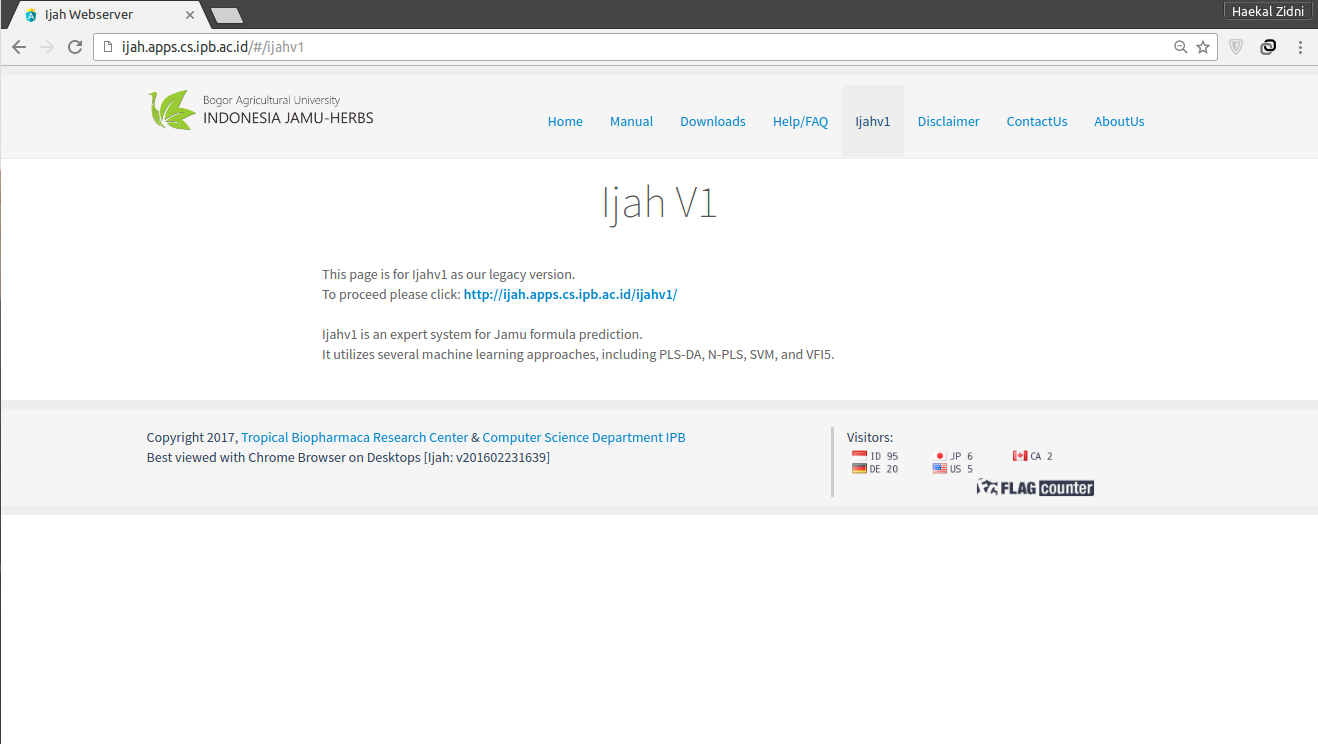
\includegraphics[scale=0.3]{ijah_v1.png}
	\caption{Isi halaman menu Ijahv1}
	\label{fig:ijah_v1}
\end{figure}

Jika anda ingin mengakses Ijahv1 silakan mengunjungi \href{http://ijah.apps.cs.ipb.ac.id/ijahv1/}{\textbf{http://ijah.apps.cs.ipb.ac.id/ijahv1/}}

\section{Disclaimer}

Menu \emph{Disclaimer} berisikan pernyataan batasan \emph{responsibility} pihak Ijah Webserver atas penggunaan hasil \emph{output} dari Ijah Webserver.

\begin{figure}[H]
	\centering
	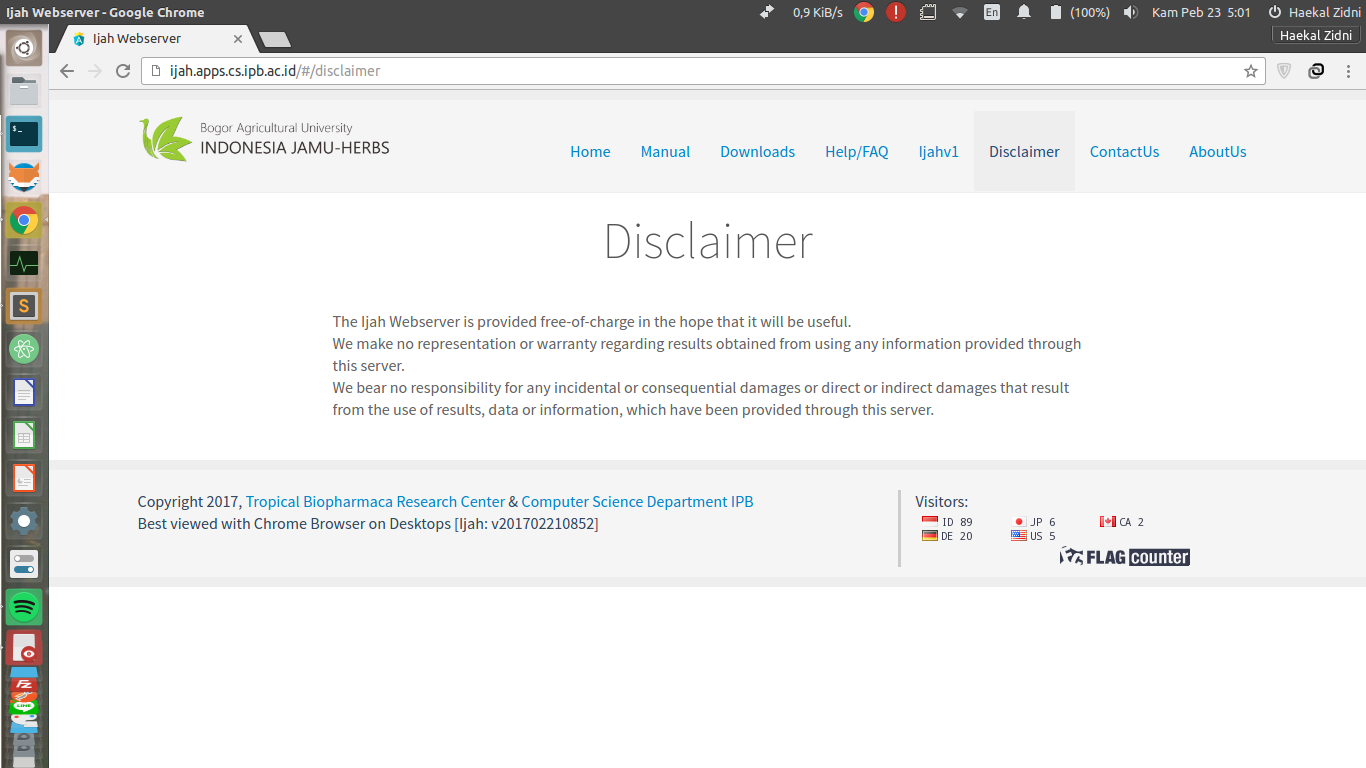
\includegraphics[scale=0.3]{ijah_disclaimer.png}
	\caption{Isi halaman Disclaimer}
	\label{fig:ijah_disclaimer}
\end{figure}

Terjemahan dari isi halaman Disclaimer yaitu:

\textit{``Ijah Webserver ini gratis, dengan harapan dapat membantu banyak pihak. Namun kami tidak menjamin akibat dari penggunaan informasi dari Webserver ini. Dan kami tidak bertanggungjawab atas insiden atau kerusakan baik langsung maupun tidak langsung yang diakibatkan oleh penggunaan data atau informasi yang kami sediakan di Webserver ini.''}


\section{ContactUs} \label{ContactUs}

Menu \emph{ContactUs} merupakan sarana komunikasi antara pengguna dengan tim pengembang Ijah Webserver. Dengan mengisikan tanggapan/keluhan/saran pada form Contact Us, tanggapan anda akan terkirim ke E-mail kami.

\begin{figure}[H]
	\centering
	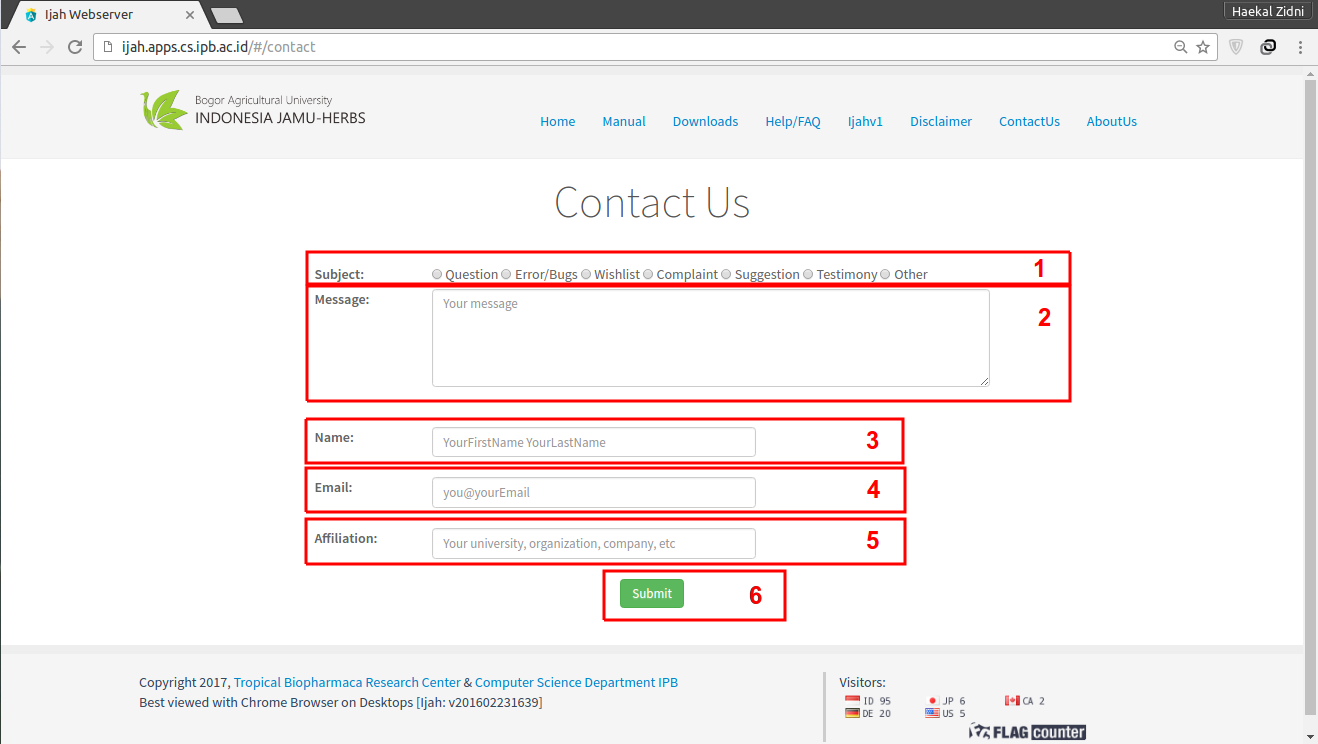
\includegraphics[scale=0.3]{ijah_contact_page.png}
	\caption{Halaman ContactUs pada Ijah Webserver:
	(1) \hyperref[subject]{Pemilihan Subject};
	(2) \hyperref[message]{Message box};
	(3) \hyperref[personal data]{Name box};
	(4) \hyperref[personal data]{E-mail box};
	(5) \hyperref[personal data]{Affiliation box};
	(6) \hyperref[submit]{Tombol Submit};
	}
	\label{fig:ijah_contact_page}
\end{figure}

	\subsection{Topik} \label{subject}
	Pada bagian \emph{Subject} anda akan memilih topik tanggapan anda 
	\begin{itemize}
	\item \textbf{Question:} mengajukan pertanyaan.
	\item \textbf{Error/Bugs:} memberitahukan adanya kesalahan.
	\item \textbf{Wishlist:} menyampaikan saran fitur apa yang diinginkan pada versi selanjutnya.
	\item \textbf{Complaint:} menyampaikan keluhan dalam penggunaan.
	\item \textbf{Suggestion:} memberikan saran.
	\item \textbf{Testimony:} memberikan testimoni tentang Ijah Webserver.
	\item \textbf{Other:} untuk menyampaikan hal lain yang tidak termasuk dalam kategori diatas.
	\end{itemize}

	\subsection{Isi Pesan} \label{message}
	Isikan pesan anda pada bagian \emph{Message}. Jumlah karakter tidak dibatasi, jadi mohon untuk tidak menggunakan singkatan jika tidak diperlukan demi memudahkan tim kami dalam membaca tanggapan anda. 


	\subsection{Isi Data Diri Anda} \label{personal data}
	Setelah menuliskan tanggapan, silakan isi data diri anda, nama pada bagian \emph{Name}, alamat E\-mail anda pada bagian \emph{E\-mail}, dan afiliasi anda (organisasi, universitas, atau perusahaan) pada bagian \emph{Affiliation}.

	\textbf{Penting:} Nama dan alamat E-mail \emph{wajib} diisi. 

	\subsection{Kirim Tanggapan} \label{submit}
	Setelah semua data terisi lengkap, tekan \textbf{Submit} dan tanggapan anda akan terkirim.

\section{AboutUs}

Menu \emph{AboutUs} berisi info tentang tim pengembang Ijah Webserver

\begin{figure}[H]
	\centering
	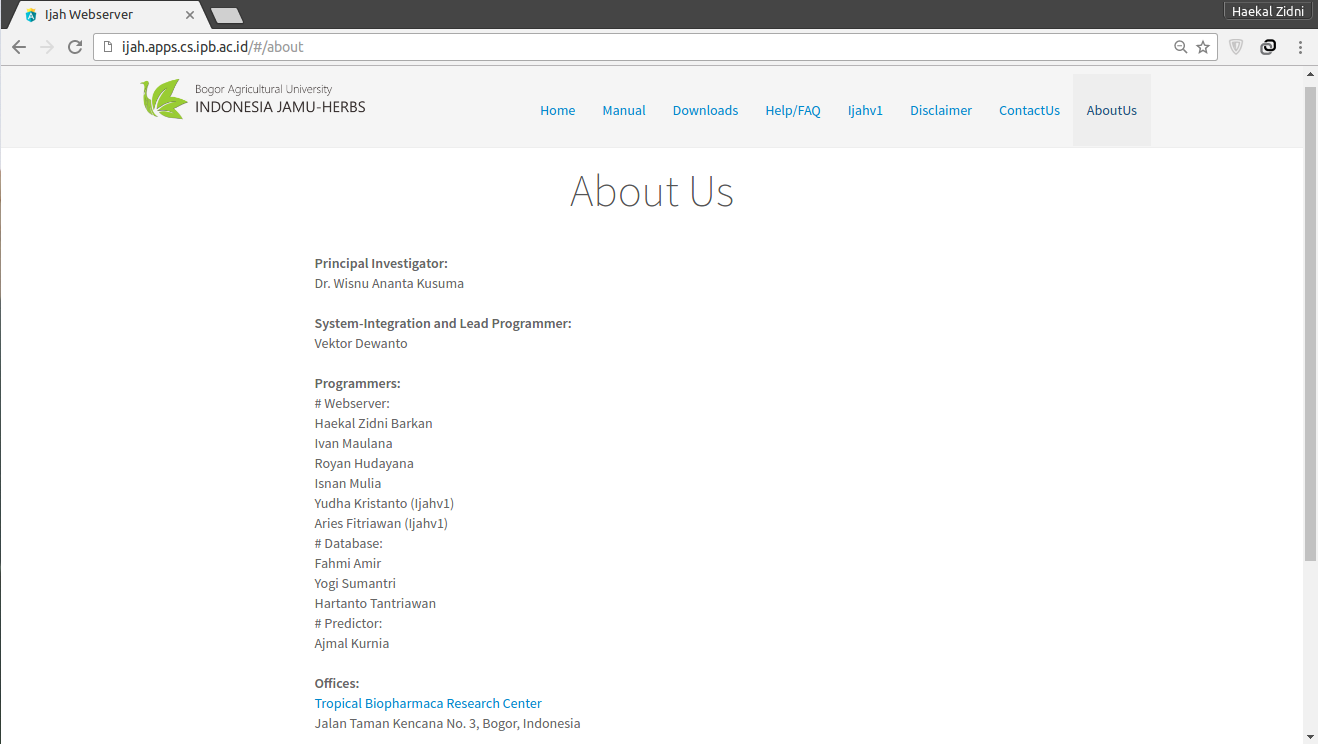
\includegraphics[scale=0.3]{ijah_about.png}
	\caption{Isi halaman About Us}
	\label{fig:ijah_about}
\end{figure}

Tim pengembang Ijah Webserver yaitu:

\begin{itemize}
\item Principal Investigator:\\ 
Dr. Wisnu Ananta Kusuma

\item System-Integration and Lead Programmer:\\
Vektor Dewanto

\item Programmers:\\
\# Webserver:
\begin{itemize}
\item Haekal Zidni Barkan
\item Ivan Maulana
\item Royan Hudayana
\item Isnan Mulia
\item Yudha Kristanto (Ijahv1)
\item Aries Fitriawan (Ijahv1)
\end{itemize}
\# Database:
\begin{itemize}
\item Fahmi Amir
\item Yogi Sumantri
\item Hartanto Tantriawan
\end{itemize}
\# Predictor:
\begin{itemize}
\item Ajmal Kurnia
\end{itemize}
\end{itemize}

% \emph{Use case} ini melibatkan hanya satu sisi yaitu \emph{Drug-side} saja. pada \emph{use case} ini, input dari salah satu \emph{drug-side} (Plant atau Compound) harus ada.

% \section{Plant Search Only}

% Pada contoh ini, input dari \emph{drug-side} berupa tanaman (Plant). Contoh ini mencari dari tanaman yang diinputkan, apa saja senyawa yang terkandung dalam tanaman itu, dan senyawa tersebut dapat berkhasiat untuk penyakit apa melalui protein apa.

% \subsection{Input}
% \begin{figure}[H]
% 	\centering
% 	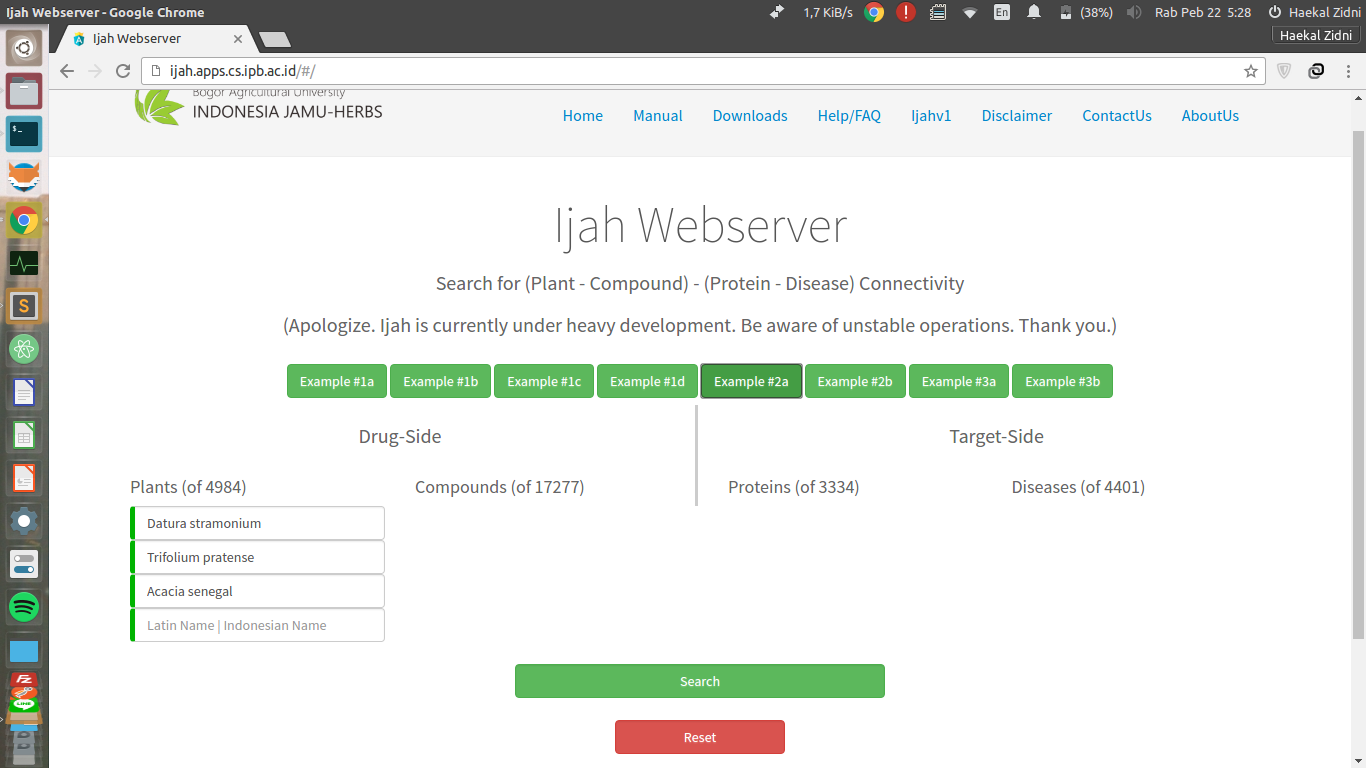
\includegraphics[scale=0.3]{example_2a.png}
% 	\caption{Contoh \emph{use case} input Plant Search Only}
% 	\label{fig:example_2a}
% \end{figure}

% Seperti yang telah dibahas pada bab sebelumnya, untuk jenis \emph{use case} ini tombol hanya bertuliskan \textbf{Search}, bukan Search and Predict seperti \emph{use case} sebelumnya.

% \subsection{Output}
% Output pada contoh \emph{search} dari 3 jenis tanaman ini adalah sebagai berikut, dimulai dari \emph{Connectivity Graph Output}

% \begin{figure}[H]
% 	\centering
% 	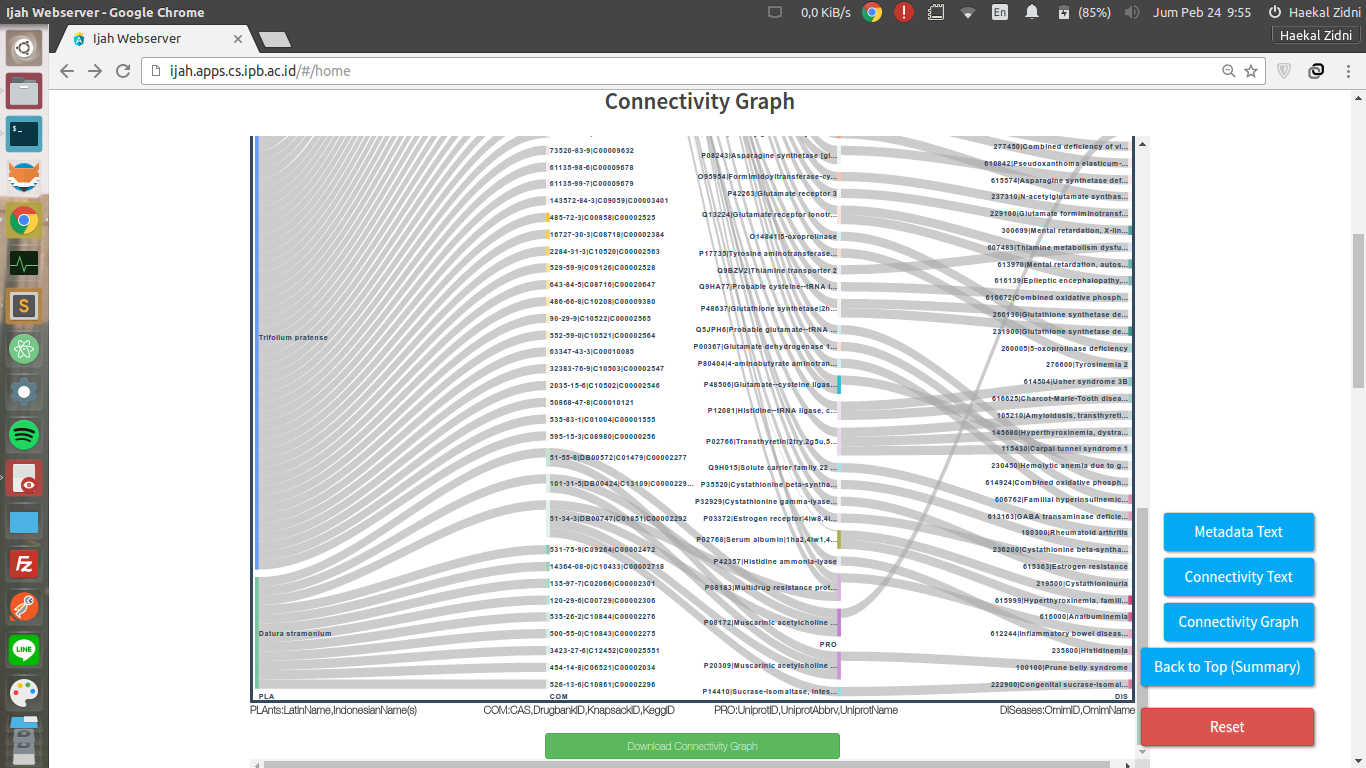
\includegraphics[scale=0.3]{ijah_example_2a_graph.png}
% 	\caption{Connectivity Graph Output pada use case Plant Search Only}
% 	\label{fig:ijah_example_2a_output}
% \end{figure}

% Graf yang dihasilkan kali ini cukup besar karena menampilkan semua penyakit yang terkait dengan seluruh senyawa yang dikandung tanaman-tanaman tersebut. Karena contoh ini menampilkan semua yang terkait dengan tanaman yang diinputkan.

% Hasil \emph{Connectivity Text Output} untuk contoh ini:

% \begin{figure}[H]
% 	\centering
% 	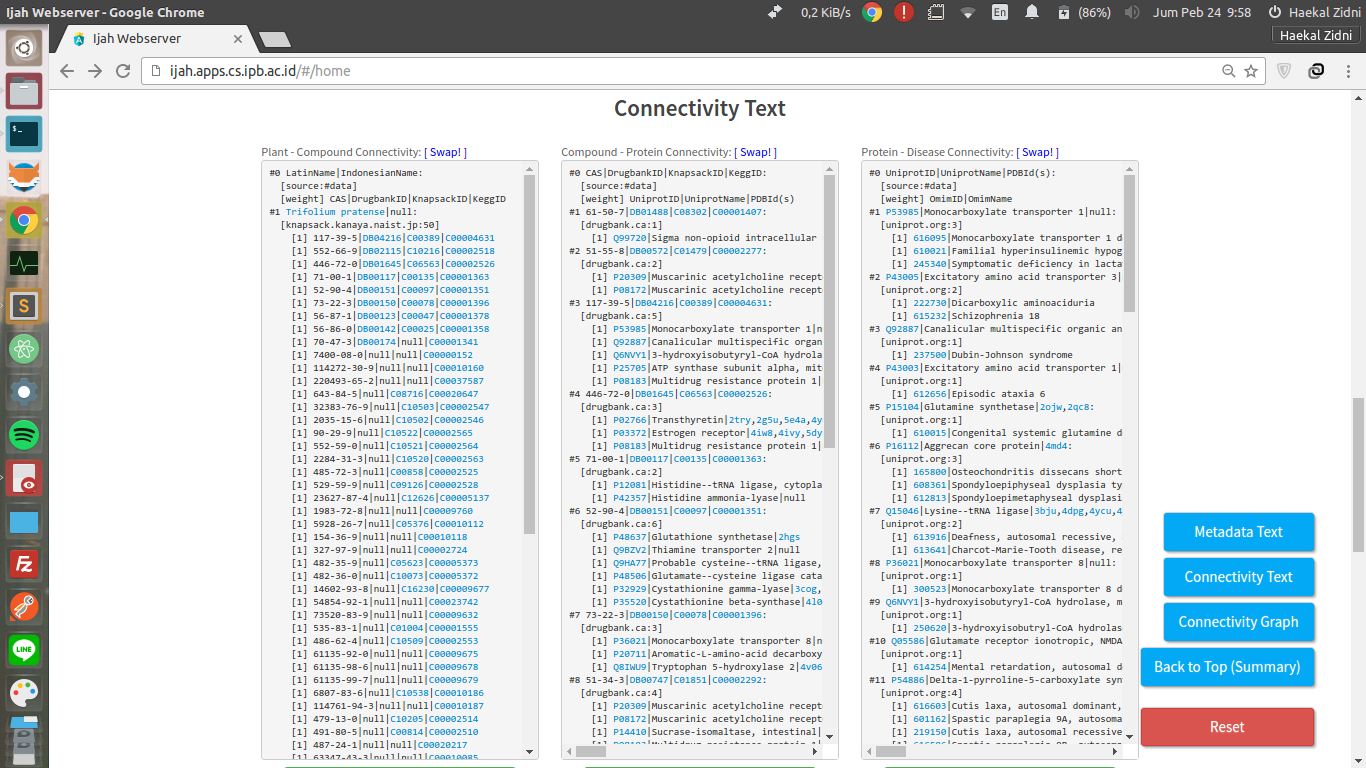
\includegraphics[scale=0.3]{ijah_example_2a_text.png}
% 	\caption{Connectivity Text Output pada use case Plant Search Only}
% 	\label{fig:ijah_example_2a_text}
% \end{figure}

% Hasil \emph{Metadata Text Output} untuk contoh ini:

% \begin{figure}[H]
% 	\centering
% 	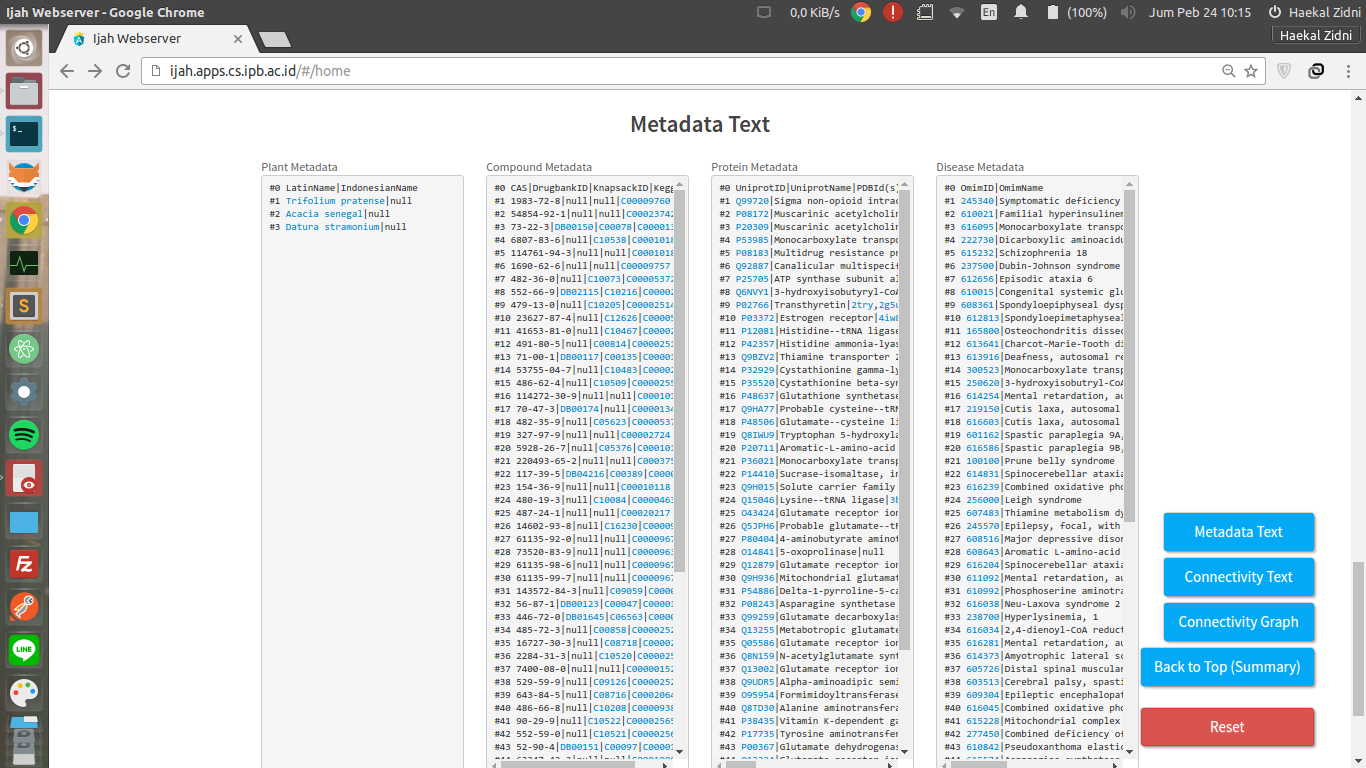
\includegraphics[scale=0.3]{ijah_example_2a_meta.png}
% 	\caption{Metadata Text Output pada use case Plant Search Only}
% 	\label{fig:ijah_example_2a_meta}
% \end{figure}

% \section{Compound Search Only}
% Contoh lain dari \emph{use case} Drug-Side Only yaitu Compound Search Only dimana perbedaannya hanya pada input, yaitu menginputkan senyawa (Compound) untuk mencari semua (Plant, Protein, Disease) yang terkait dengan senyawa yang diinputkan.

